\documentclass[11pt,a4paper]{jsarticle}
%
\usepackage{amsmath,amssymb}
\usepackage{bm}
\usepackage{graphicx}
\usepackage{ascmac}
\usepackage{atbegshi}
\usepackage{geometry} % 追加: 余白を一時的に0にするため
\usepackage{listings} % ソースコード表示のために追加
\usepackage{float}
\usepackage{tcolorbox}
\newtcbox{\code}[1][]{
  colback=gray!10!white,
  colframe=gray!20!white,
  boxrule=0.5pt,
  left=2pt,right=2pt,top=1pt,bottom=1pt,
  box align=base,
  fontupper=\ttfamily
}
% 簡易コード表示用マクロ(本文中で\textttt{...}を使えるようにする)
\newcommand{\textttt}[1]{\texttt{#1}}
%ここからソースコードの表示に関する設定
\lstset{
  basicstyle={\ttfamily},
  identifierstyle={\small},
  commentstyle={\smallitshape},
  keywordstyle={\small\bfseries},
  ndkeywordstyle={\small},
  stringstyle={\small\ttfamily},
  frame={tb},
  breaklines=true,
  columns=[l]{fullflexible},
  numbers=left,
  xrightmargin=0zw,
  xleftmargin=3zw,
  numberstyle={\scriptsize},
  stepnumber=1,
  numbersep=1zw,
  lineskip=-0.5ex
}
\renewcommand{\lstlistingname}{ソースコード} % キャプションを「ソースコード」に変更
%ここまでソースコードの表示に関する設定
\newcommand{\myPdfAuthor}{平田爽馬/HIRATA,Soma}
\newcommand{\myPdfTitle}{電源回路の基礎実験}
\AtBeginShipoutFirst{\special{pdf:tounicode EUC-UCS2}} % pLaTeXの内部漢字コードがEUCの場合
\AtBeginDvi{\special{pdf:docinfo <<
 /Author   (\myPdfAuthor)
 /Title    (\myPdfTitle)>>}}
%
\setlength{\textwidth}{\fullwidth}
\setlength{\textheight}{40\baselineskip}
\addtolength{\textheight}{\topskip}
\setlength{\voffset}{-0.2in}
\setlength{\topmargin}{0pt}
\setlength{\headheight}{0pt}
\setlength{\headsep}{0pt}
%
\newcommand{\divergence}{\mathrm{div}\,}  %ダイバージェンス
\newcommand{\grad}{\mathrm{grad}\,}  %グラディエント
\newcommand{\rot}{\mathrm{rot}\,}  %ローテーション
%
\title{\myPdfTitle}
\author{5E25番 平田爽馬}
\date{}
\begin{document}
%\maketitle%タイトルを挿入したくない場合は,消す
%
%
\section{目的}
ダイオードを用いた電源回路にといて,交流を直流にする整流回路や整流波形から脈動分を除去する平滑回路の動作を調べる.
また,応用回路として,3端子レギュレータ,チョッパ電源回路についての動作も調べ理解を深める.

\section{原理}
一般に.電源回路はトランスと整流回路,平滑回路から構成される.
以降,整流回路と平滑回路,応用回路について簡単に説明する.

\subsection{電源回路の基礎}
図\ref{fig1}のように直流で動作する電子回路を動作させるためには,交流である商用電源から整流・平滑により直流にする交流-直流変換の電圧源や電池など,不安定な直流電圧を安定化電源により安定した電圧に変換して供給する.\\
本節では,直流-直流変換の電源回路(安定化電源)の種類と特徴を解説し,交流から直流に変換する整流・平滑回路について説明する.

\begin{figure}[H]
\centering
\includegraphics[width=85mm]{./fig/fig1.eps}
\caption{負荷である電子回路への電源構成}
\label{fig1}
\end{figure}

\subsubsection{電源回路の種類と特徴}
不安定な直流電圧から安定した直流電圧に変換する安定化電源は,図\ref{fig2}に示すように方式や回路構成によって分類できる.
\begin{figure}[H]
\centering
\includegraphics[width=85mm]{./fig/fig2.eps}
\caption{電源回路(安定化電源)の分類}
\label{fig2}
\end{figure}

また,電源回路の基本的な構成は図\ref{fig3}のようになり,出力の電圧検出回路の出力と基準電圧回路の出力を制御回路により比較して,出力トランジスタなどのエネルギー変換素子を制御することで$V_o$を一定にする.

\begin{figure}[H]
\centering
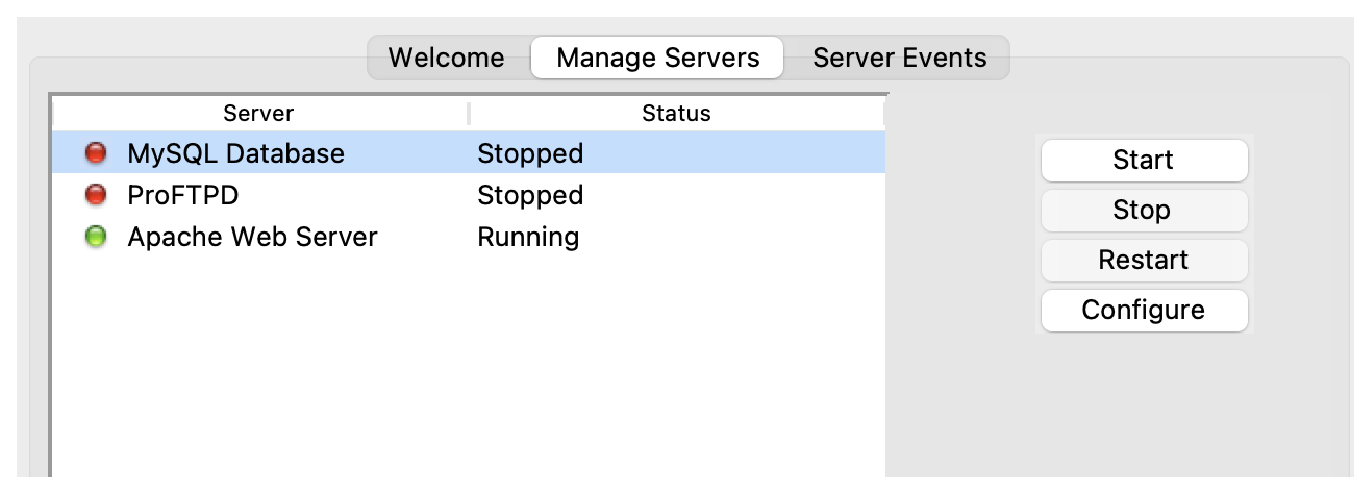
\includegraphics[width=100mm]{./fig/fig3.eps}
\caption{電源回路の基本構成}
\label{fig3}
\end{figure}

\subsubsection*{リニア方式およびスイッチング方式の特徴}
図\ref{fig2}のリニア方式とスイッチング方式についてそれぞれ特徴を述べる.
\paragraph{リニア方式}\quad\\
リニア方式は,制御回路とエネルギー変換素子である出力トランジスタは線形アナログ動作領域のみで動作して一定の出力電源を発生する.回路構成により山とレギュレータとシリーズレギュレータに分けられる.\\
リニア方式の電源には次のような特徴がある.
\begin{itemize}
\item 高い電源電圧から低い出力電圧に変換する降圧型のみである.
\item 出力電流=入力電流となるため,電力損失は入力と出力の電圧差に比例する.
\item 出力トランジスタを線形アナログ動作領域で制御するため出力にノイズが発生しない.
\item 出力トランジスタとトランジスタを中心に構成した制御回路や基準電圧で回路を構成できるため半導体に集積可能である.
\end{itemize}

\paragraph{スイッチング方式}\quad\\
スイッチング方式には,エネルギー変換素子としてインダクタやキャパシタと出力トランジスタを用い,制御回路により入力側電源からの電流を出力トランジスタでオン・オフさせることでインダクタやキャパシタに蓄積するエネルギーを制御して,一定の電圧を出力する.

スイッチング方式は出力トランジスタをオン・オフさせて制御することから非線形回路となる.
そして,エネルギー変換阻止部分の構成により,入力電源電圧に対して低い電圧を出力する降圧型,h逆に高い電圧を出力する昇圧型,降圧型と昇圧型の両方を動作する昇降圧型,入力電源い対して逆の極性の電源を出力する斑点型に分けられる.\\
スイッチング方式の電源には次のような特徴がある.
\begin{itemize}
\item 入力電力と出力電力をほぼ等しくすることができて電力損失が少なく高効率である.
\item 出力トランジスタのオン・オフにより出力にノイズが生じる.
\item エネルギー変換素子としてインダクタやキャパシタを使用するので半導体に集積するのは容易ではなく,電源回路構成によって複雑になる.
\end{itemize}
\end{document}